% Use only LaTeX2e, calling the article.cls class and 12-point type.

\documentclass[12pt]{article}

\bibliographystyle{science}
% Users of the {thebibliography} environment or BibTeX should use the
% scicite.sty package, downloadable from *Science* at
% www.sciencemag.org/about/authors/prep/TeX_help/ .
% This package should properly format in-text
% reference calls and reference-list numbers.

\usepackage{scicite}
\usepackage{graphicx,subcaption,lineno}

% Use times if you have the font installed; otherwise, comment out the
% following line.

\usepackage{times}

% The preamble here sets up a lot of new/revised commands and
% environments.  It's annoying, but please do *not* try to strip these
% out into a separate .sty file (which could lead to the loss of some
% information when we convert the file to other formats).  Instead, keep
% them in the preamble of your main LaTeX source file.


% The following parameters seem to provide a reasonable page setup.

\topmargin 0.0cm
\oddsidemargin 0.2cm
\textwidth 16cm 
\textheight 21cm
\footskip 1.0cm


%The next command sets up an environment for the abstract to your paper.

\newenvironment{sciabstract}{%
\begin{quote} \bf}
{\end{quote}}


% If your reference list includes text notes as well as references,
% include the following line; otherwise, comment it out.

%\renewcommand\refname{References and Notes}

% The following lines set up an environment for the last note in the
% reference list, which commonly includes acknowledgments of funding,
% help, etc.  It's intended for users of BibTeX or the {thebibliography}
% environment.  Users who are hand-coding their references at the end
% using a list environment such as {enumerate} can simply add another
% item at the end, and it will be numbered automatically.

\newcounter{lastnote}
\newenvironment{scilastnote}{%
\setcounter{lastnote}{\value{enumiv}}%
\addtocounter{lastnote}{+1}%
\begin{list}%
{\arabic{lastnote}.}
{\setlength{\leftmargin}{.22in}}
{\setlength{\labelsep}{.5em}}}
{\end{list}}

\renewcommand{\thesubfigure}{\Alph{subfigure}}
% Include your paper's title here

\title{Death and taxa: time-invariant differences in mammal species duration}


% Place the author information here.  Please hand-code the contact
% information and notecalls; do *not* use \footnote commands.  Let the
% author contact information appear immediately below the author names
% as shown.  We would also prefer that you don't change the type-size
% settings shown here.

\author
{Peter D Smits$^{1\ast}$\\
\\
\normalsize{$^{1}$Committee on Evolutionary Biology, University of Chicago,}\\
\normalsize{1025 E. 57th Street, Culver Hall 402, Chicago, IL 60637, USA}\\
}

% Include the date command, but leave its argument blank.

\date{}



%%%%%%%%%%%%%%%%% END OF PREAMBLE %%%%%%%%%%%%%%%%



\begin{document} 

% Double-space the manuscript.

\baselineskip24pt

% Make the title.

\maketitle 
%\linenumbers
%\modulolinenumbers[2]

% Place your abstract within the special {sciabstract} environment.

\begin{sciabstract}
 Determining which biological traits influence differences in extinction risk is vital for understanding the differential diversification of life and for making predictions about species' vulnerability to anthropogenic impacts. Here I present a hierarchical Bayesian survival model of North American Cenozoic mammal species durations as predicted by species-level ecological factors, time of origination, and phylogenetic relationships. I find support for the ``survival of the unspecialized'' as a time-invariant generalization of trait-based extinction risk. Furthermore, I find that phylogenetic and temporal effects are both substantial factors associated with differences in species durations. The current biodiversity crisis is partially incongruous with previous patterns. This incongruity implies that the either the fossil record is a poor predictor of risk in the modern world, or that the current biodiversity crisis has transitioned into a state comparable to the great mass extinctions in Earth history.
\end{sciabstract}

Why extinction risk varies among species remains one of the most fundamental questions in paleobiology and conservation biology \cite{Simpson1944,VanValen1973,Raup1994,Quental2013,Wagner2014b}. To address this issue, I test for associations between extinction risk and multiple species-level traits during times of background extinction and in the modern world; which traits have time-invariant effects on species duration; and whether extinction is age-independent. I approach these questions together by using a model of species duration whose parameter estimates act as direct tests of these questions. Cenozoic mammals are an ideal focus for this study because their fossil record is well sampled and well resolved both temporally and spatially, and because individual species ecology and taxonomic position are generally understood \cite{Alroy2009,Liow2008,Smith2004,Quental2013,Simpson1944,Tomiya2013,Marcot2014}. 

The species-level traits studied here are bioprovince occupancy, body mass, and both dietary and locomotor categories. These traits are related to aspects of a species' adaptive zone such as population density, expected range size, potential prey, and dispersal ability \cite{Smith2004,Jernvall2004}. It is expected that species with larger geographic ranges have lower extinction rates than species with smaller geographic ranges \cite{Jablonski1986,Roy2009c}; however, how traits more directly related to species--environment interactions play a role is more nebulous.

Body size is a complex trait related to many life history characteristics. There are three general hypotheses of how body size may effect extinction risk: 1) positive effect where an increase in body size causes an increase in extinction risk, potentially due to associated decrease in reproductive rate or similar \cite{Liow2008,Liow2009}; 2) negative effect where an increase in body size causes a decrease in extinction risk because of an expected positive relationship between body size and geographic range; and 3) no effect of body size on extinction risk \cite{Tomiya2013}. 

The strongest expectation of the effect of dietary category on extinction risk is that omnivores will have the lowest extinction risk of all species. This hypothesis is based on the long standing ``survival of the unspecialized'' hypothesis where more generalist species (e.g. omnivores) have greater survival than specialist species (e.g. carnivores/herbivores) \cite{Liow2004a,Simpson1944}. It has also been observed that both carnivores and herbivores have greater diversification rates than omnivores, with herbivores diversifying faster than carnivores \cite{Price2012}. How this result translates into expectations of differences in extinction risk is currently unknown. In modern taxa, higher trophic levels (e.g. carnivores versus herbivores) have been associated with an increase in extinction risk, most likely because of human extermination of top predators \cite{Liow2009,Purvis2000a}. 

Similarly, there are few simple expectations of how locomotor category may effect extinction risk. During the Cenozoic there was a shift at the Paleogene/Neogene boundary from predominately closed to predominately open environments \cite{Blois2009,Janis1993a}. Based on this observation, a simple prediction is that arboreal taxa will have the greatest extinction risk of all, with both scansorial and ground dwelling taxa having lower extinction risks. 

Time-invariant factors are those that have a constant directional effect even if the magnitude varies. Because change in the magnitude of extinction risk is not necessarily the best indicator of a shift from background to mass extinction \cite{Wang2003}, it is better to look for changes in either the direction of selection, the loss of a selective pressure, or the appearance of novel selective pressures \cite{Jablonski1986}.

I use a hierarchical Bayesian survival model of species duration as predicted by the covariates of interest along with species' temporal and phylogenetic context. Species duration, in 2 My bins, was modeled as being drawn from either an exponential or Weibull distribution parameterized as a hierarchical regression \cite{Gelman2013d}. The exponential is a special case of the Weibull where the shape parameter, $\alpha$, is 1 which corresponds to the Law of Constant Extinction, which states that extinction is age-independent \cite{VanValen1973}. Origination cohorts were modeled as exchangeable draws from a common normal distribution. Phylogenetic effect was modeled assuming species duration may have evolved via Brownian motion \cite{Housworth2004}. Extended explanation of the model, choice of priors, parameter estimation, and posterior predictive check results are provided in the supplementary online text. The results from the Weibull model are detailed here because this model has a better fit to the data the exponential (Fig.~\ref{fig:ppc_surv}, S1, S2).

% show results from exponential model results along side weibull results
%   make sure the signs are the same for exponential and weibull?
%     then I can show estimates together with double histograms?
%     will really help explain the actual results
%   do as two histograms in the same panel for the posterior predictive checks!
%     probably just in supplement
%   results are consistent with which hypotheses?
Species with greater bioprovince occupancy are found to be associated with lower extinction risk than taxa with smaller bioprovince occupancy (Mean \(\beta_{occupancy} = -0.53\), Std \(= 0.08\)). This is consistent with prior expectations. Body size has nearly zero association with expected duration (Mean \(\beta_{size} = -0.05\), Std \(= 0.05\)), a similar result to some previous studies \cite{Tomiya2013}. However, previous studies were performed at the generic-level and were unable to determine how body size may effect species level extinction, as the effect of either extinction or speciation cannot be distinguished \cite{Tomiya2013,Liow2008}.

Some clear patterns emerge from the pairwise differences in effect of each dietary category on expected duration (Fig.~\ref{fig:trait_est}). Consistent with expectations from the ``survival of the unspecialized'' hypothesis \cite{Liow2004a,Simpson1944}, omnivory appears to be associated with the lowest expected extinction risk. Carnivory is associated a greater expected duration than either herbivory or insectivory, but a greater expected extinction risk then omnivory. Finally, herbivory and insectivory have approximately equal effects on expected duration. Given previous results, these results imply that carnivores have a greater origination rate than omnivores \cite{Price2012}. These results also imply that herbivores, which have the greatest extinction risk, must also have a very high origination rate in order to have the greatest diversification rate among these three categories \cite{Price2012}. 

For locomotor category, both scansoriality and ground dwelling life habitat are associated with a greater expected duration than arboreality (Fig.~\ref{fig:trait_est}). Scansorial and ground dwelling life habits also have approximately equal expected effects on extinction risk.  This is consistent with the expectation that arboreality will confer greater extinction risk due to the loss of associated environment with the shift from open to closed habitat at the Paleogene/Neogene boundary \cite{Blois2009}.

Of the three sources of variance present in the model, individual species variance accounts for approximately 80\% of the observed, unmodeled variance (Fig.~\ref{fig:vpc}). Both cohort and phylogenetic effects account for the other 20\% of the observed variance. This result means that extinction risk has both temporal and phylogenetic aspects, as both contribute greater than 0\% of the observed variability in the data \cite{Housworth2004}.

% decrease in extinction risk with time is known previous result
% plot S(t) for each cohort with posterior predictive checks as panels?
%   this is probably very useful way of depicting variance in cohort survival functions
% two part figure 
%   Exponential and Weibull fit to S(t)
%   facet grid with each cohort S(t)
%     show Exponential and Weibull fits per cohort, two overlaping colors
The estimates for the individual cohort effects show a weak pattern of greater extinction risk in older Cenozoic cohorts compared to younger cohorts (Fig.~\ref{fig:eff_cohort}). This potential slowdown in extinction risk is consistent with previous analyses of marine invertebrates \cite{Raup1982a,Foote2003} and mammals \cite{Alroy2010c,Alroy2000g}. There are two prevailing hypotheses as to the cause of this slowdown: 1) extinction risk is constant within, but varies between, clades so over time clades with low extinction rates increases in proportion of total diversity thus bringing down expected extinction risk; or 2) over time taxa increase in mean fitness and thus decrease in expected extinction risk \cite{Raup1982a}. The observed decrease in extinction risk with age, along with the variance partitioning results (Fig.~\ref{fig:vpc}) are consistent with both of these hypotheses with neither being more ``important'' than the other. 

Interestingly, the shift from older cohorts with a higher extinction risk to younger cohorts with lower extinction risk is approximately at the Paleogene--Neogene boundary. Given the association with arboreality (a heritable trait) and increased extinction risk (Fig.~\ref{fig:trait_est}), the decrease in expected extinction risk over time might relate to the preferential loss of arboreal taxa over the Cenozoic. However, because the model used here does not allow for change in time-invariant effects, I cannot identify whether this boundary is associated with a shift in the direction or magnitude of the expected effect of arboreality on extinction risk.

When these results are compared to factors contributing to increased extinction risk in extant mammals, there are some in congruencies. As expected, large range size is always associated with lower extinction risk in the modern world \cite{Fritz2009,Fritz2010b,Liow2009,Purvis2000a}. While my analysis found body size to have almost no time-invariant effect on extinction risk, this is not necessarily the case in extant mammals where increased body size is associated with increased extinction risk \cite{Liow2009,Purvis2000a}. However, this pattern is partially clade dependent \cite{Fritz2009}. As stated earlier, higher trophic levels have been found to be associated with greater extinction risk in extant mammals \cite{Purvis2000a,Liow2009}. In contrast, I found that omnivores and carnivores have a lower expected extinction risk than either insectivores or herbivores (Fig.~\ref{fig:trait_est}). Finally, phylogeny has been found to be a good predictor of differences in extinction risk in extant mammals as certain clades are at much higher risks than others \cite{Fritz2010b}. This effect seems much greater in the Recent than for the whole Cenozoic, implying that current extinction risk is more phylogenetically concentrated than in previous mammal extinctions. 

Whether these incongruities are within the standard range of time-variant effects is unknown, though my comparisons do imply that current processes are different from those studied here. These incongruities imply that the fossil record may not provide a guide for conservation biology. However, this is not a model of what makes taxa vulnerable during mass extinctions and that may account for these incongruities, assuming mass extinctions are qualitatively different than background extinction \cite{Jablonski1986}. These results would also be inapplicable if the current biodiversity crisis is qualitatively different from either background or mass extinction as preserved in the fossil record.

By modeling how different ecologies and historical factors effect a species' expected extinction risk, it is possible to better understand what processes may have driven the resulting pattern of selection (i.e. diversity). This analysis finds broad support for the ``survival of the unspecialized'' hypothesis \cite{Simpson1944,Liow2004a} as a time-invariant generalization about extinction risk. I also find that there are substantial effects of both cohort and phylogeny on extinction risk, which supports the idea that the decrease in extinction risk \cite{Raup1982a} over time has both temporal and phylogenetic components. Additionally, I found evidence of increasing extinction risk with species age, the cause of which is unknown. These results, when compared to current mammal extinction risk factors, support the hypothesis that the current biodiversity crisis is qualitatively different from ``normal'' extinction, possibly because the current biodiversity crisis is a mass extinction event.


\bibliography{newbib,packages}

% Following is a new environment, {scilastnote}, that's defined in the
% preamble and that allows authors to add a reference at the end of the
% list that's not signaled in the text; such references are used in
% *Science* for acknowledgments of funding, help, etc.

\begin{scilastnote}
%\item Materials and methods are available as supplementary materials on Science Online. 
\item P.D.S would like to thank M. Foote, K. Angielczyk, R. Ree, P.D. Polly for discussion; N. Pierrehumbert, E. Sander, L. Southcott for draft comments; and J. Alroy and the Fossilworks/Paleobiology Database for data accumulation, management, and availability. This is Paleobiology Database publication number XXX.
\end{scilastnote}


% For your review copy (i.e., the file you initially send in for
% evaluation), you can use the {figure} environment and the
% \includegraphics command to stream your figures into the text, placing
% all figures at the end.  For the final, revised manuscript for
% acceptance and production, however, PostScript or other graphics
% should not be streamed into your compliled file.  Instead, set
% captions as simple paragraphs (with a \noindent tag), setting them
% off from the rest of the text with a \clearpage as shown  below, and
% submit figures as separate files according to the Art Department's
% instructions.

\clearpage


\begin{figure}[ht]
  \centering
  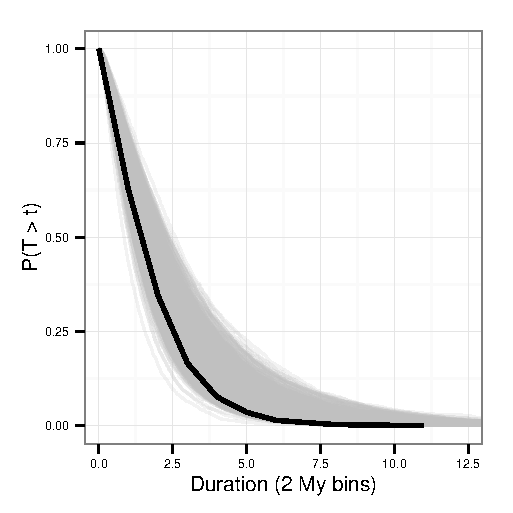
\includegraphics[height = 0.5\textheight, width = \textwidth, keepaspectratio = true]{figure/survival_function}
  \caption{Comparison of estimates of the empirical survival function (black) and survival functions from 1000 simulated data sets using the fitted model (dark grey). The survival function is the probability that a species with duration \(t\) will not have gone extinct. Simulated data sets were generated by drawing parameter values randomly from their estimated posteriors and using the observed covariate information to estimate durations for all the observed species. On the left are the results from the exponential survival model, while on the right are the results the Weibull model.}
  \label{fig:ppc_surv}
\end{figure}

\begin{figure}[ht]
  \centering
  \begin{subfigure}[b]{0.4\textwidth}
    \caption{}
    \includegraphics[height = 0.5\textheight, width = \textwidth, keepaspectratio = true]{figure/loco_diff_est}
    \label{subfig:loco}
  \end{subfigure}
  \begin{subfigure}[b]{0.4\textwidth}
    \caption{}
    \includegraphics[height = 0.5\textheight, width = \textwidth, keepaspectratio = true]{figure/diet_diff_est}
    \label{subfig:diet}
  \end{subfigure}
  \caption{Pairwise differences in effect of the locomotor (\textbf{A}) and dietary categories (\textbf{B}) on expected duration from 1000 samples from the posterior distribution. Comparisons of locomotor categories, from top to bottom (\textbf{A}), are: arboreal versus ground dwelling, arboreal versus scansorial, and ground dwelling versus scansorial. For dietary category, from top to bottom (\textbf{B}): carnivore versus herbivore, carnivore versus insectivore, carnivore versus omnivore, herbivore versus insectivore, herbivore versus omnivore, and insectivore versus omnivore. Values to the left indicate that the first category is expected to have a greater duration than the second, while values to the right indicate that the first category is expected to have a shorter duration.}
  \label{fig:trait_est}
\end{figure}

\begin{figure}[ht]
  \centering
  \includegraphics[height = 0.5\textheight, width = \textwidth, keepaspectratio = true]{figure/cohort_est}
  \caption{Summaries of posterior estimates of individual cohort effect depicted as medians and 80\% credible intervals. High values correspond to shorter species durations while lower values correspond to greater species durations compared to the mean duration. Lines are placed at the middle of the 2 My origination cohorts.}
  \label{fig:eff_cohort}
\end{figure}

\begin{figure}[ht]
  \centering
  \includegraphics[height = 0.5\textheight, width = \textwidth, keepaspectratio = true]{figure/variance_est}
  \caption{Estimates of the variance partitioning coefficients for the three different sources of variance: species, cohort, and phylogeny. Higher values correspond to greater contribution to total observed variance. Each of the estimates is a distribution of 1000 approximating simulations due to the model's non-normally distributed errors.}
  \label{fig:vpc}
\end{figure}

\end{document}
